\documentclass{letask}

\begin{document}
\begin{titlepage}
\center % Center everything on the page
 
%----------------------------------------------------------------------------------------
%	HEADING SECTIONS
%----------------------------------------------------------------------------------------

\textsc{\LARGE Московский\\[-0.2cm]Физико-Технический Институт\\[0.1cm]\large (государственный университет)}\\[1.5cm] % Name of your university/college
\textsc{\Large Кафедра общей физики}\\[0.1cm] % Major heading such as course name
\textsc{\large Лабораторная работа \textnumero  4.5.2}\\[0.5cm] % Minor heading such as course title

%----------------------------------------------------------------------------------------
%	TITLE SECTION
%----------------------------------------------------------------------------------------

\HRule
\\[0.4cm]
{ \huge \bfseries Интерференция\\[0.2cm]
лазерного излучения}
\\[0.6cm] % Title of your document
\HRule
\\[1.5cm]


 
%----------------------------------------------------------------------------------------
%	AUTHOR SECTION
%----------------------------------------------------------------------------------------


	\begin{flushleft} \large
		\textsf{Студент}
		
		Северилов Павел \\[-0.15cm]
		671 группа
	\end{flushleft}


\begin{bottompar}
	\begin{center}
		
\includegraphics[width = 80 mm]{logo.jpg}
	\end{center}
	{\large \today}

\end{bottompar}
\vfill % Fill the rest of the page with whitespace

\end{titlepage}

\textbf{Цель работы:}
познакомиться с явлением интерференции в тонких плёнках (полосы равной толщины) на примере колец Ньютона и с методикой интерференционных измерений кривизны стеклянной поверхности.

\textbf{В работе используются:} измерительный микроскоп с опак-иллюминатором; плосковыпуклая линза; пластинка из черного стекла; ртутная лампа ДРШ; щель; линзы; призма прямого зрения; объектная шкала.

\section{Теоретическая часть}

\begin{wrapfigure}[12]{r}{5 cm}
\label{img: lens}
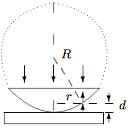
\includegraphics[width = 4.5 cm]{lens}
\caption{Запись голограммы точки}
\end{wrapfigure}
В нашей установке кольца Ньютона образуются при интерференции световых волн, отраженных от границ тонкой воздушной прослойки, заключенной между выпуклой поверхностью линзы и плоской стеклянной пластинкой (рис. \ref{img: lens}). Наблюдение ведется в отраженном свете.

Рассчитаем размеры колец Ньютона. Пусть сверху на линзу падает монохроматический параллельный пучок лучей. При вычислении разности хода можно пренебречь небольшими наклонами лучей, проходящих в тонком воздушном зазоре. Геометрическая разность хода между интерферирующими лучами равна, очевидно, $2d$, где $d$~—~толщина воздушного зазора в данном месте.

Выразим зависимость d от расстояния r до радиуса, проходящего через точку соприкосновения линзы и пластинки. Из рис. \ref{img: lens} имеем

\[
r^2 = R^2 - (R-d)^2 = 2Rd - d^2,
\]

где $R$~--~радиус кривизны выпуклой поверхности. Учитывая, что $2R \gg d$, имеем:
\[ d= \dfrac{r^2}{2R} \]

При вычислении полной разности хода учтем, что при пр отражении от оптически более плотной среды происходит изменение фазы на $\pi$. Тогда свет, отраженный от границы стекло-воздух, по сравнению со светом, отраженным от границы воздух-стекло, приобретает дополнительный фазовый сдвиг на $\pi$, что соответствует разности хода $\lambda / 2$. Полная разность хода $\Delta$ равна:
\begin{equation}
\label{eq:Delta}
\Delta = 2d + \dfrac{\lambda}{2} = \dfrac{r^2}{R} + \dfrac{\lambda}{2}.
\end{equation}

Линии постоянной разности хода представляют собой концентрические кольца с центром в точке соприкосновения. При заданном значении длины волны $\lambda$ разность хода $\Delta$ определяется толщиной воздушного зазора; интерференционные полосы являются, таким образом, линиями равной толщины.

Известно, что линии равной толщины для точечного источника света не имеют области локализации: их можно наблюдать в любом месте пространства, где пересекаются лучи, отражённые от двух поверхностей. Для протяжённого источника линии равной толщины локализованы на поверхности клина (в нашем случае на поверхности воздушной прослойки). Это означает, что при освещении системы не вполне параллельным пучком света (что практически всегда имеет место) интерференционные полосы оказываются наиболее четкими при фокусировке на верхнюю поверхность воздушного клина.

Запишем условие минимума освещенности в интерференционной картине:
\[ \Delta = (2m + 1)\dfrac{\lambda}{2}, \qquad m = 0, 1, 2, \ldots\]

Учитывая выражение (\ref{eq:Delta}), получим для радиусов темных колец:

\begin{equation}
\label{eq: dark}
r_m = \sqrt{mR \lambda} .
\end{equation} 

Для радиусов светлых колец:
\begin{equation}
\label{eq: light}
r_m = \sqrt{(2m-1)R\lambda / 2}.
\end{equation}

Таким образом, зная радиусы темных и светлых колец, с помощью (\ref{eq: dark}) и (\ref{eq: light}) можно определить $R$ по известному значению $\lambda$.

\section{Ход работы}
\begin{enumerate}
	\item Включили ртутную лампу и настроили микроскоп на кольца Ньютона в белом свете
	\item Настроили монохроматор, фокусируя на входном окне опак-иллюминатора зеленую линию. (собрали установку, как на рисунке)
	\begin{figure}[H]
		\centering
		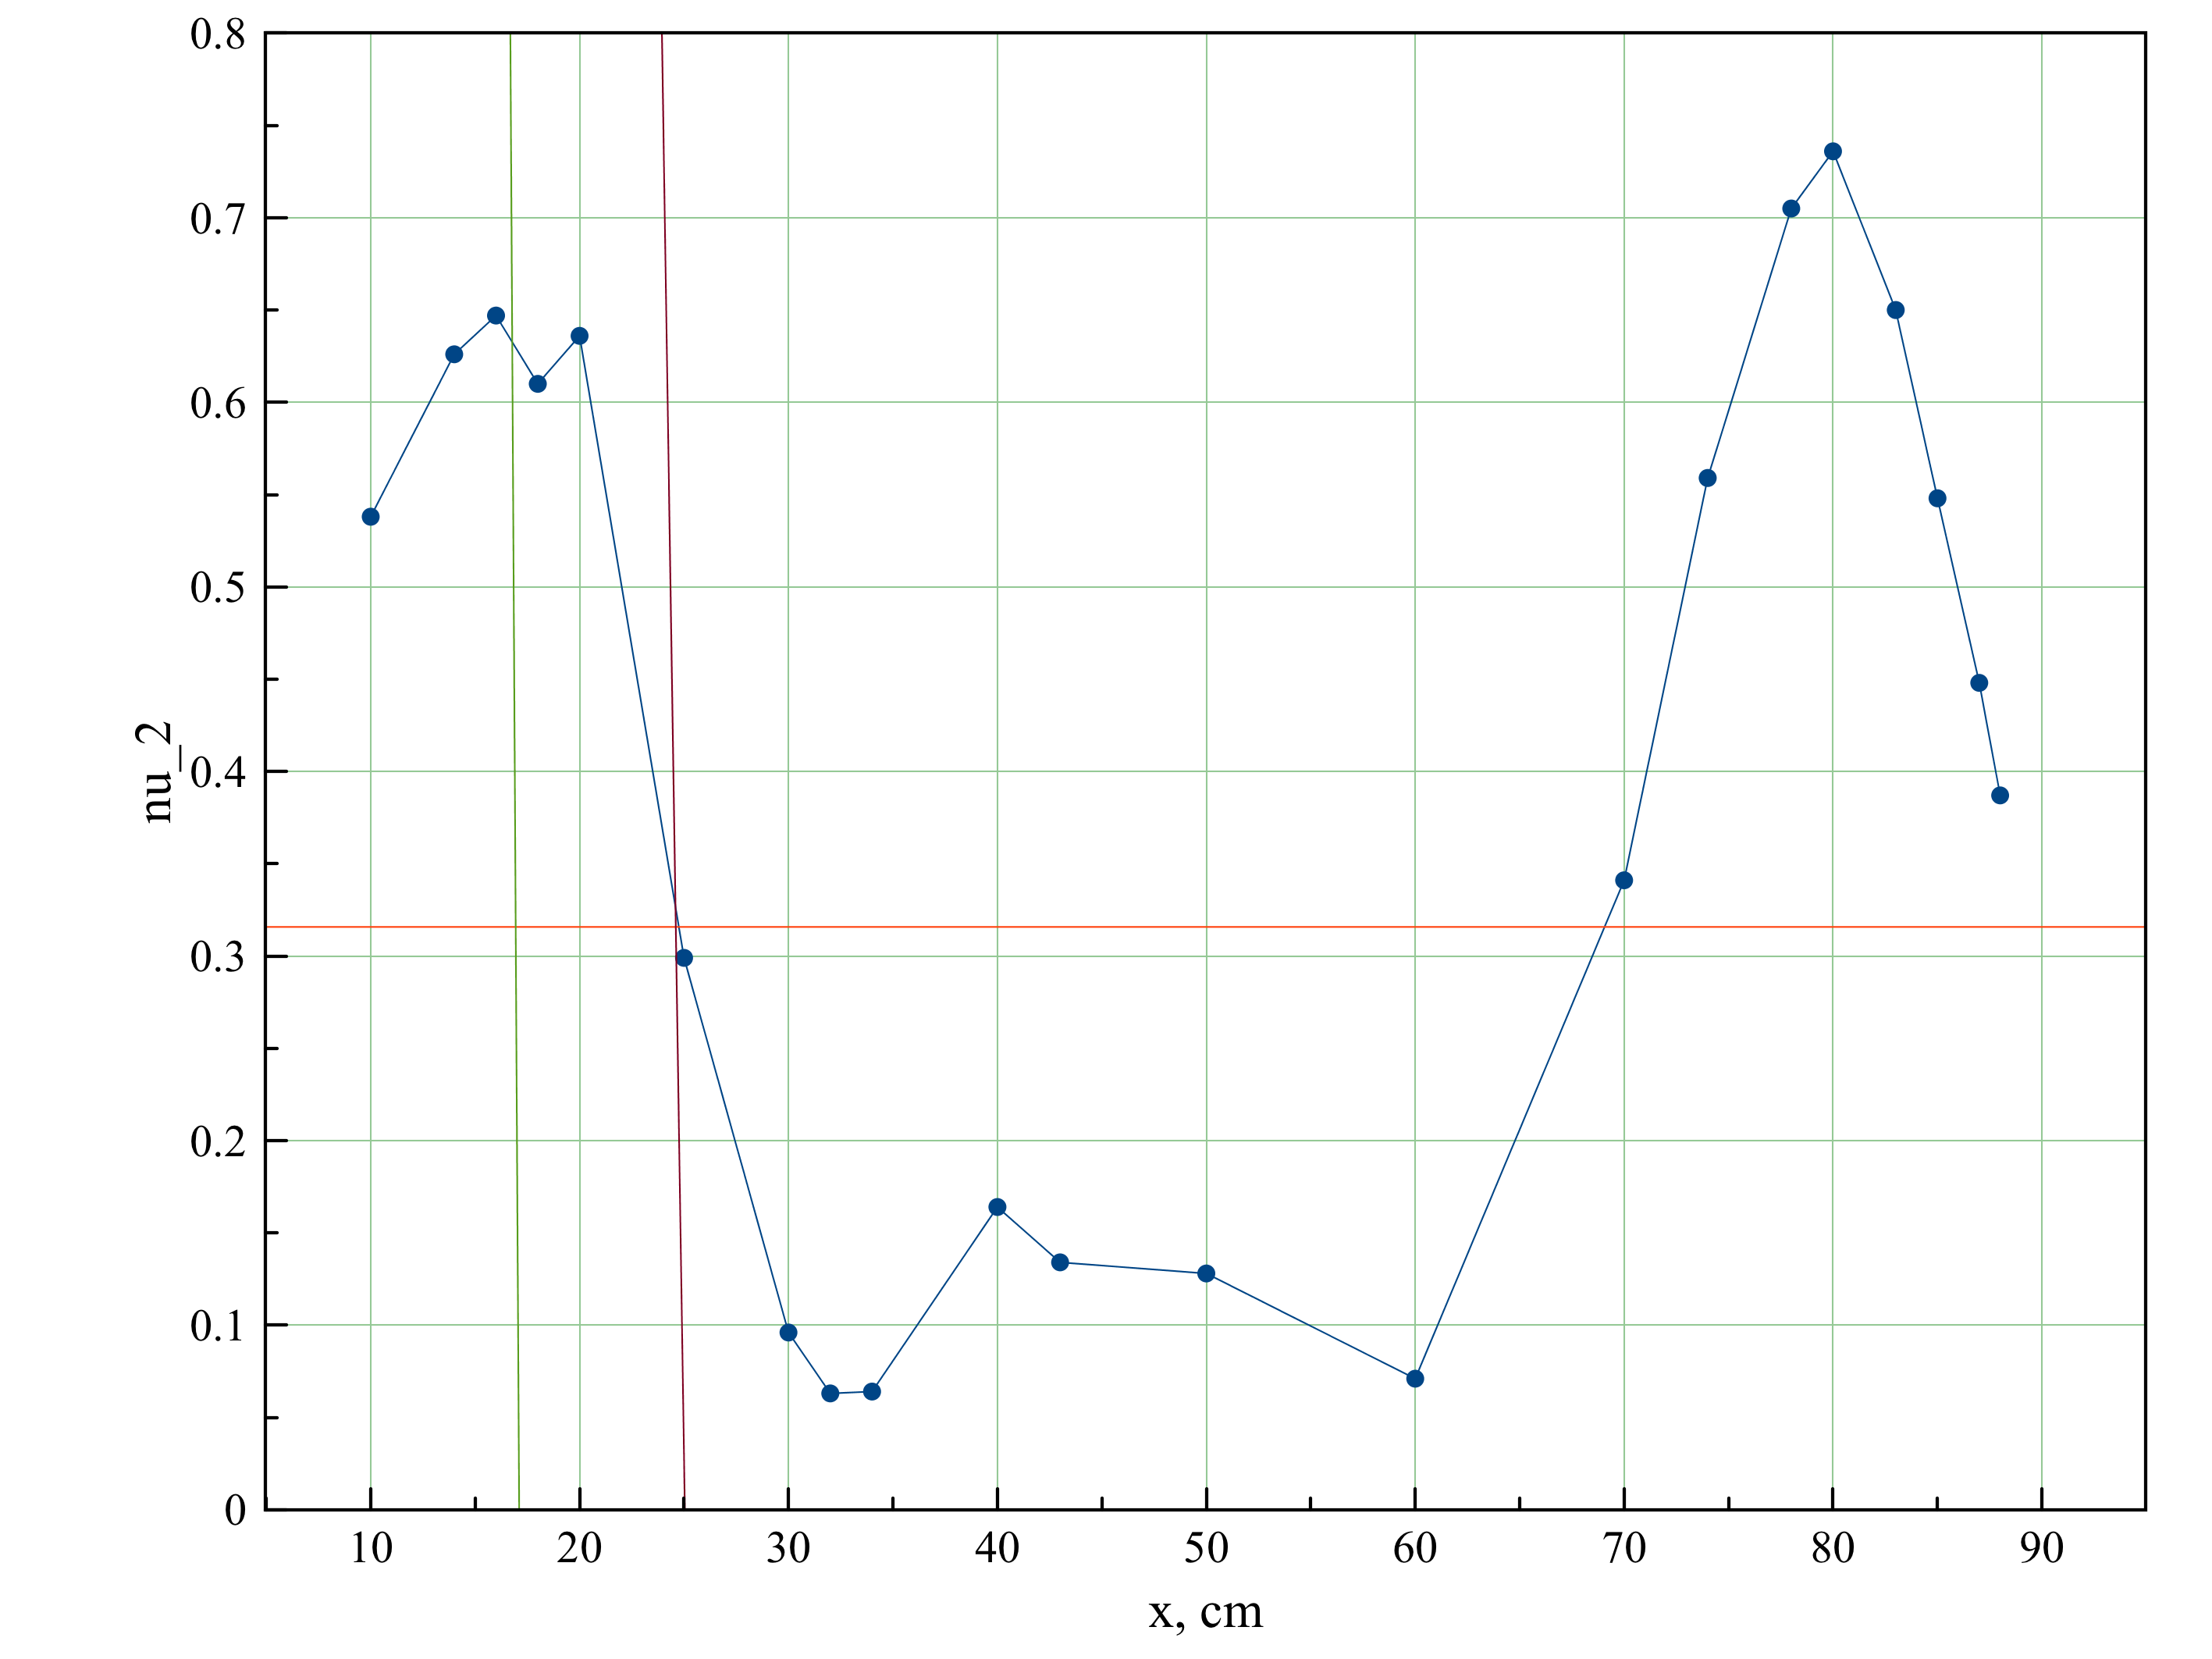
\includegraphics[width = 0.7 \lw]{2.png}
	\end{figure}
	\item Определили координаты диаметров темных и светлых колец, результаты занесли в таблицу
	\item Провели наблюдение биений для желтой и зеленой линий 
	\item Прокалибровали окулярную шкалу, используя эталонную шкалу
\end{enumerate}

\section{Отчет}

\subsection{Определение цены деления}
Для вычисления цены деления окулярной шкалы наложили на линзу калиброванную объектную шкалу размером $1 \; \mm$, для которой заранее известна цена деления. Совместив две шкалы можем оценить цену деления окулярной шкалы: на $11.35 \text{ед. шкалы}$ помещается $100$ делений ($1 \mm$), то есть цена деления окулярной шкалы равна:
\[\dfrac{1}{11.35} = 0.09 ~\mm\]

Погрешность результата: ошибка для определения ед.шкалы $\sigma = 0.4$ ед. шкалы. Тогда погрешность цены деления: $\sigma_{\text{ц.д.}} = 0.09 ~\mm\sqrt{\left(\cfrac{\sigma}{11.35}\right)^2} = 1.7\cdot 10^{-3} ~\mm$ ($\varepsilon = 3.5 \%$)


\begin{minipage}{0.55\textwidth}
\subsection{Радиусы колец}
\begin{table}[H]
\centering{
\begin{tabular}{|c|c|c|c|c|c|c|c|c|c|c|c|c|}
\hline
$m$	&$r$, дел	&$\Delta r^2, 10^{-8} \m^2$ 	&$r$, дел	&$\Delta r^2, 10^{-8} \m^2 $\\ \hline
6	&1,30	&6,53	&1,29	&6,58\\ \hline
5	&1,60	&5,23	&1,55	&5,43\\ \hline
4	&1,84	&4,28	&1,84	&4,28\\ \hline
3	&2,20	&3,05	&2,09	&3,40\\ \hline
2	&2,50	&2,18	&2,41	&2,42\\ \hline
1	&2,98	&1,09	&2,74	&1,59\\ \hline
0   &4,14	&0,00	&4,96	&0,54\\ \hline
1	&5,36	&1,21	&5,53	&1,57\\ \hline
2	&5,83	&2,31	&6,03	&2,89\\ \hline
3	&6,16	&3,31	&6,22	&3,50\\ \hline
4	&6,50	&4,51	&6,58	&4,82\\ \hline
5	&6,77	&5,60	&6,81	&5,77\\ \hline
6	&7,04	&6,81	&7,01	&6,67\\ \hline
\end{tabular}
}
\caption{Измерение радиусов темных колец}
\end{table}
\end{minipage}
~
\begin{minipage}{0.5\textwidth}
	\begin{figure}[H]
		\centering
		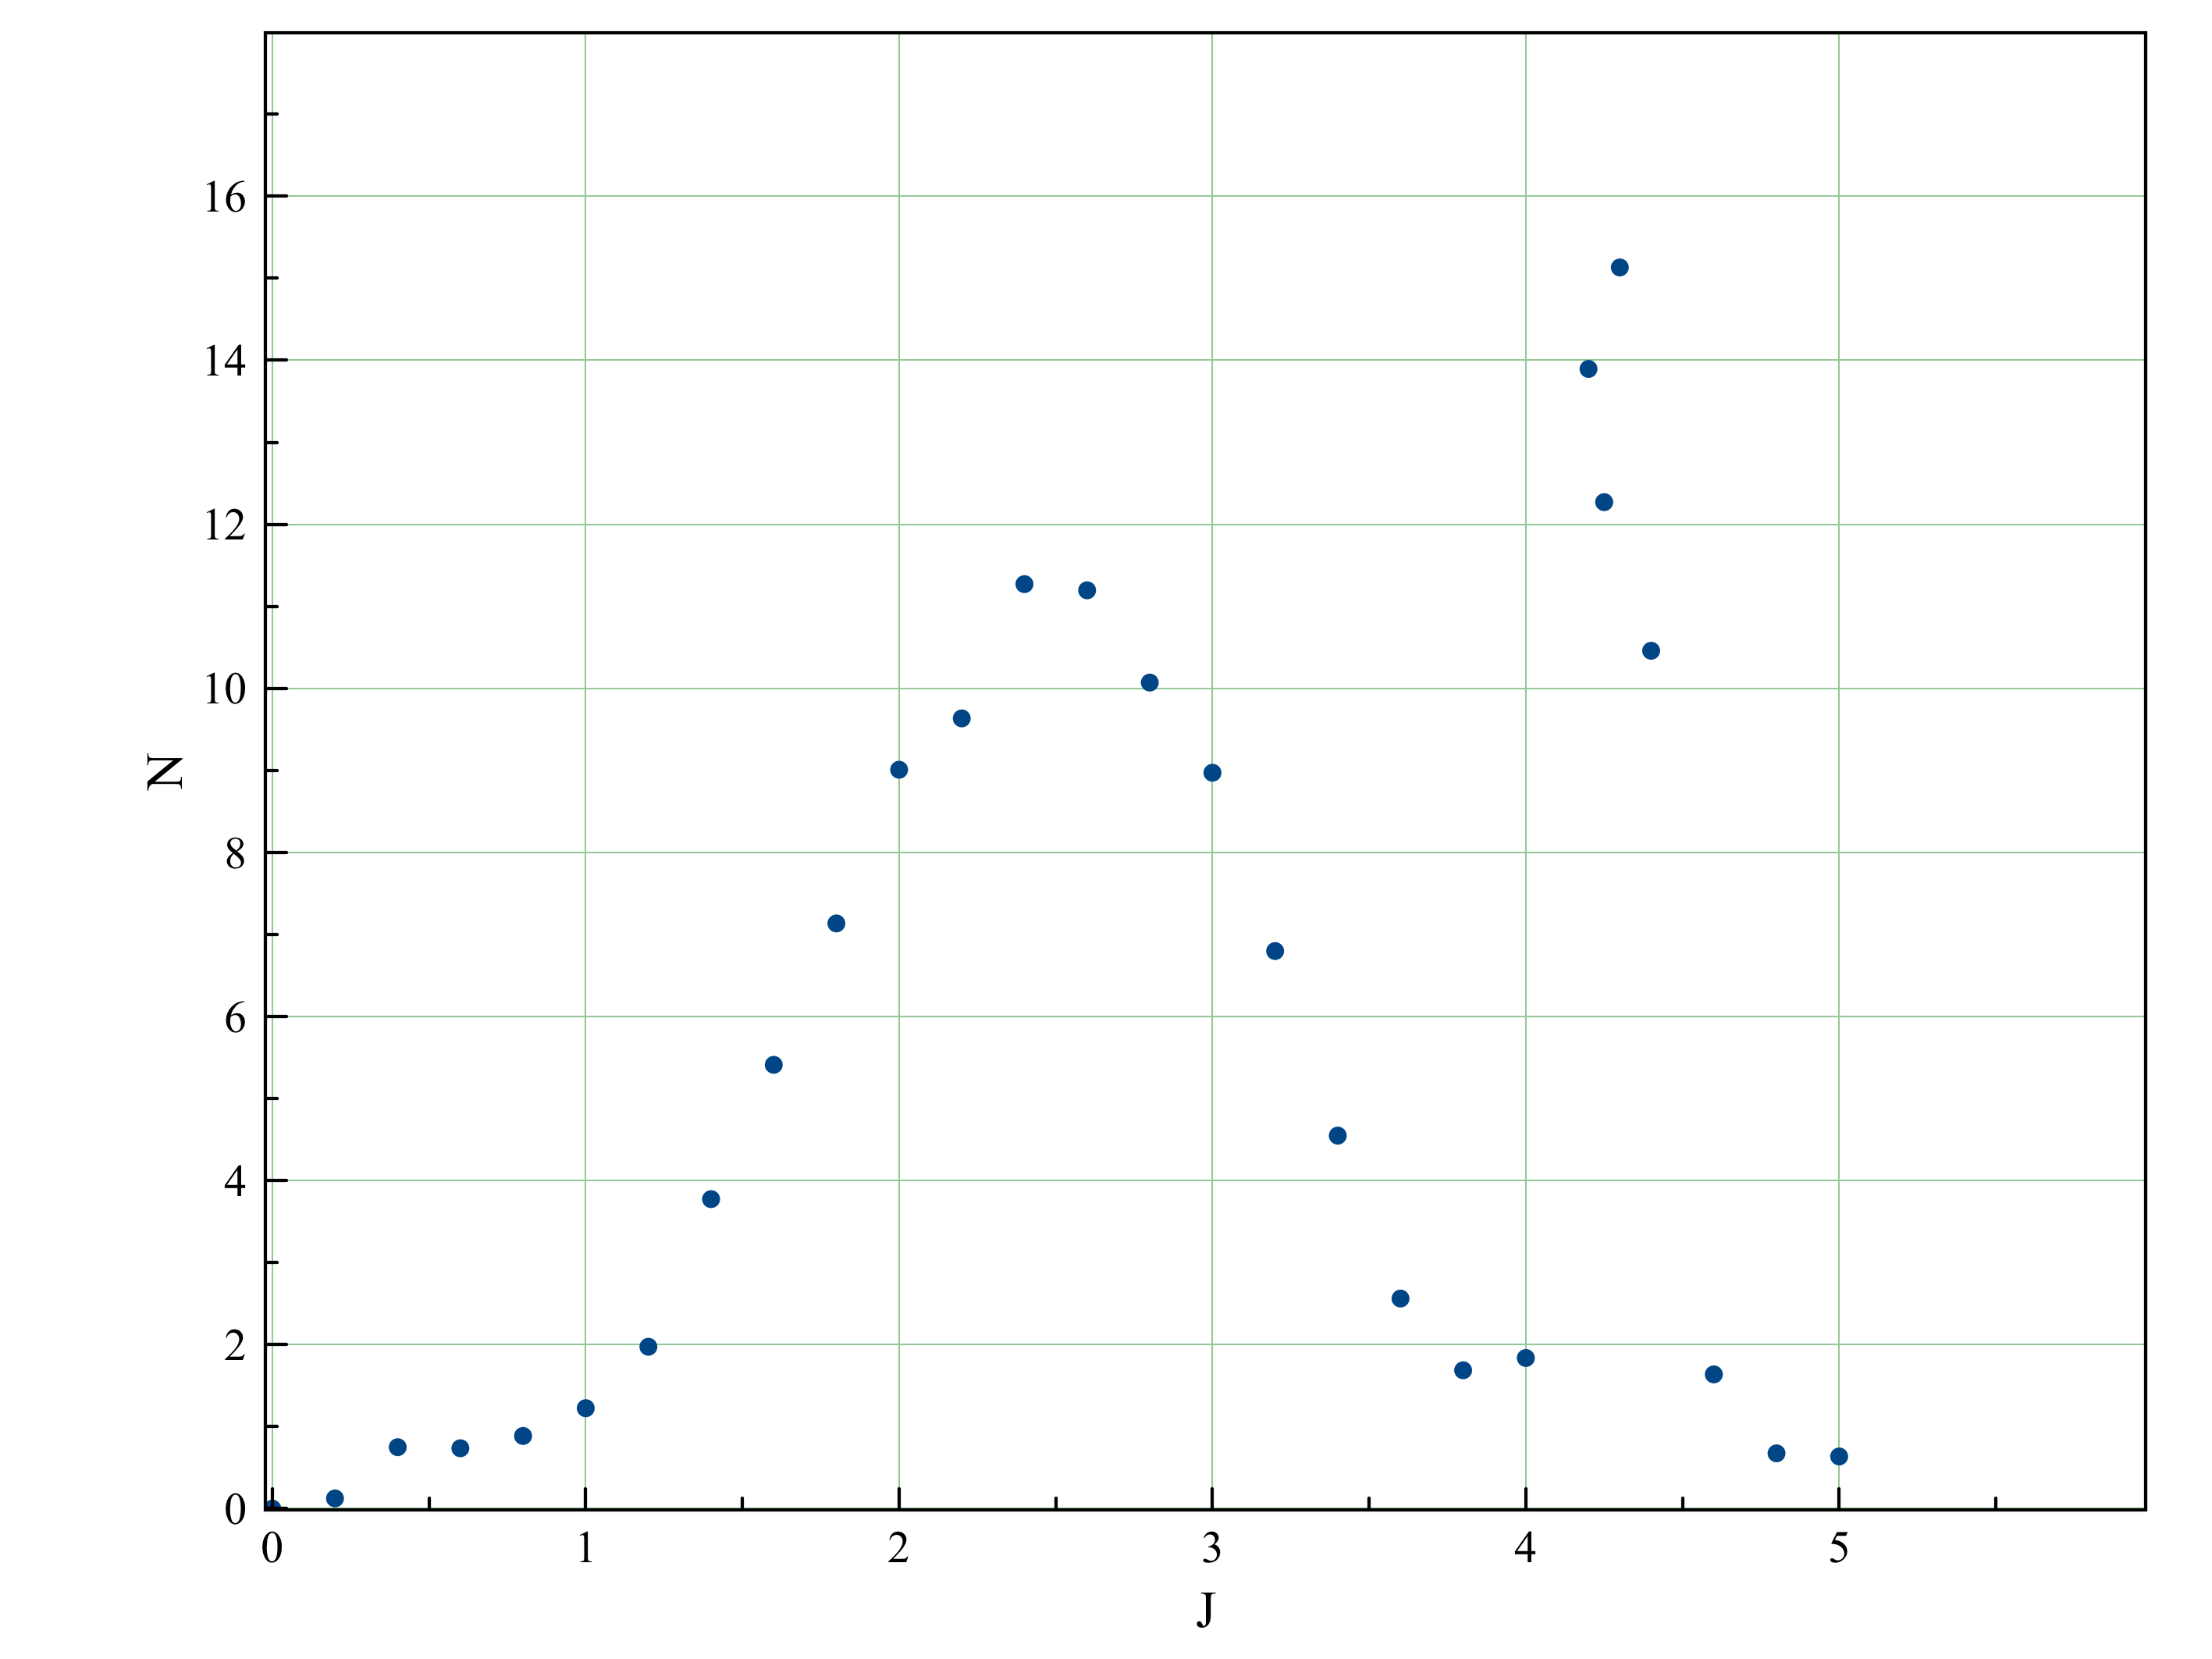
\includegraphics[width = 0.8 \lw]{1}
	\end{figure}
\end{minipage}


Построим график зависимости $r_m^2(m)$ для темных и светлых колец.

Получаем для темных колец: $r_m^2 = 1.096m$\\
Получаем для светлых колец: $r_m^2 = 1.03m - 0.422$

\begin{figure}[H]
	\centering
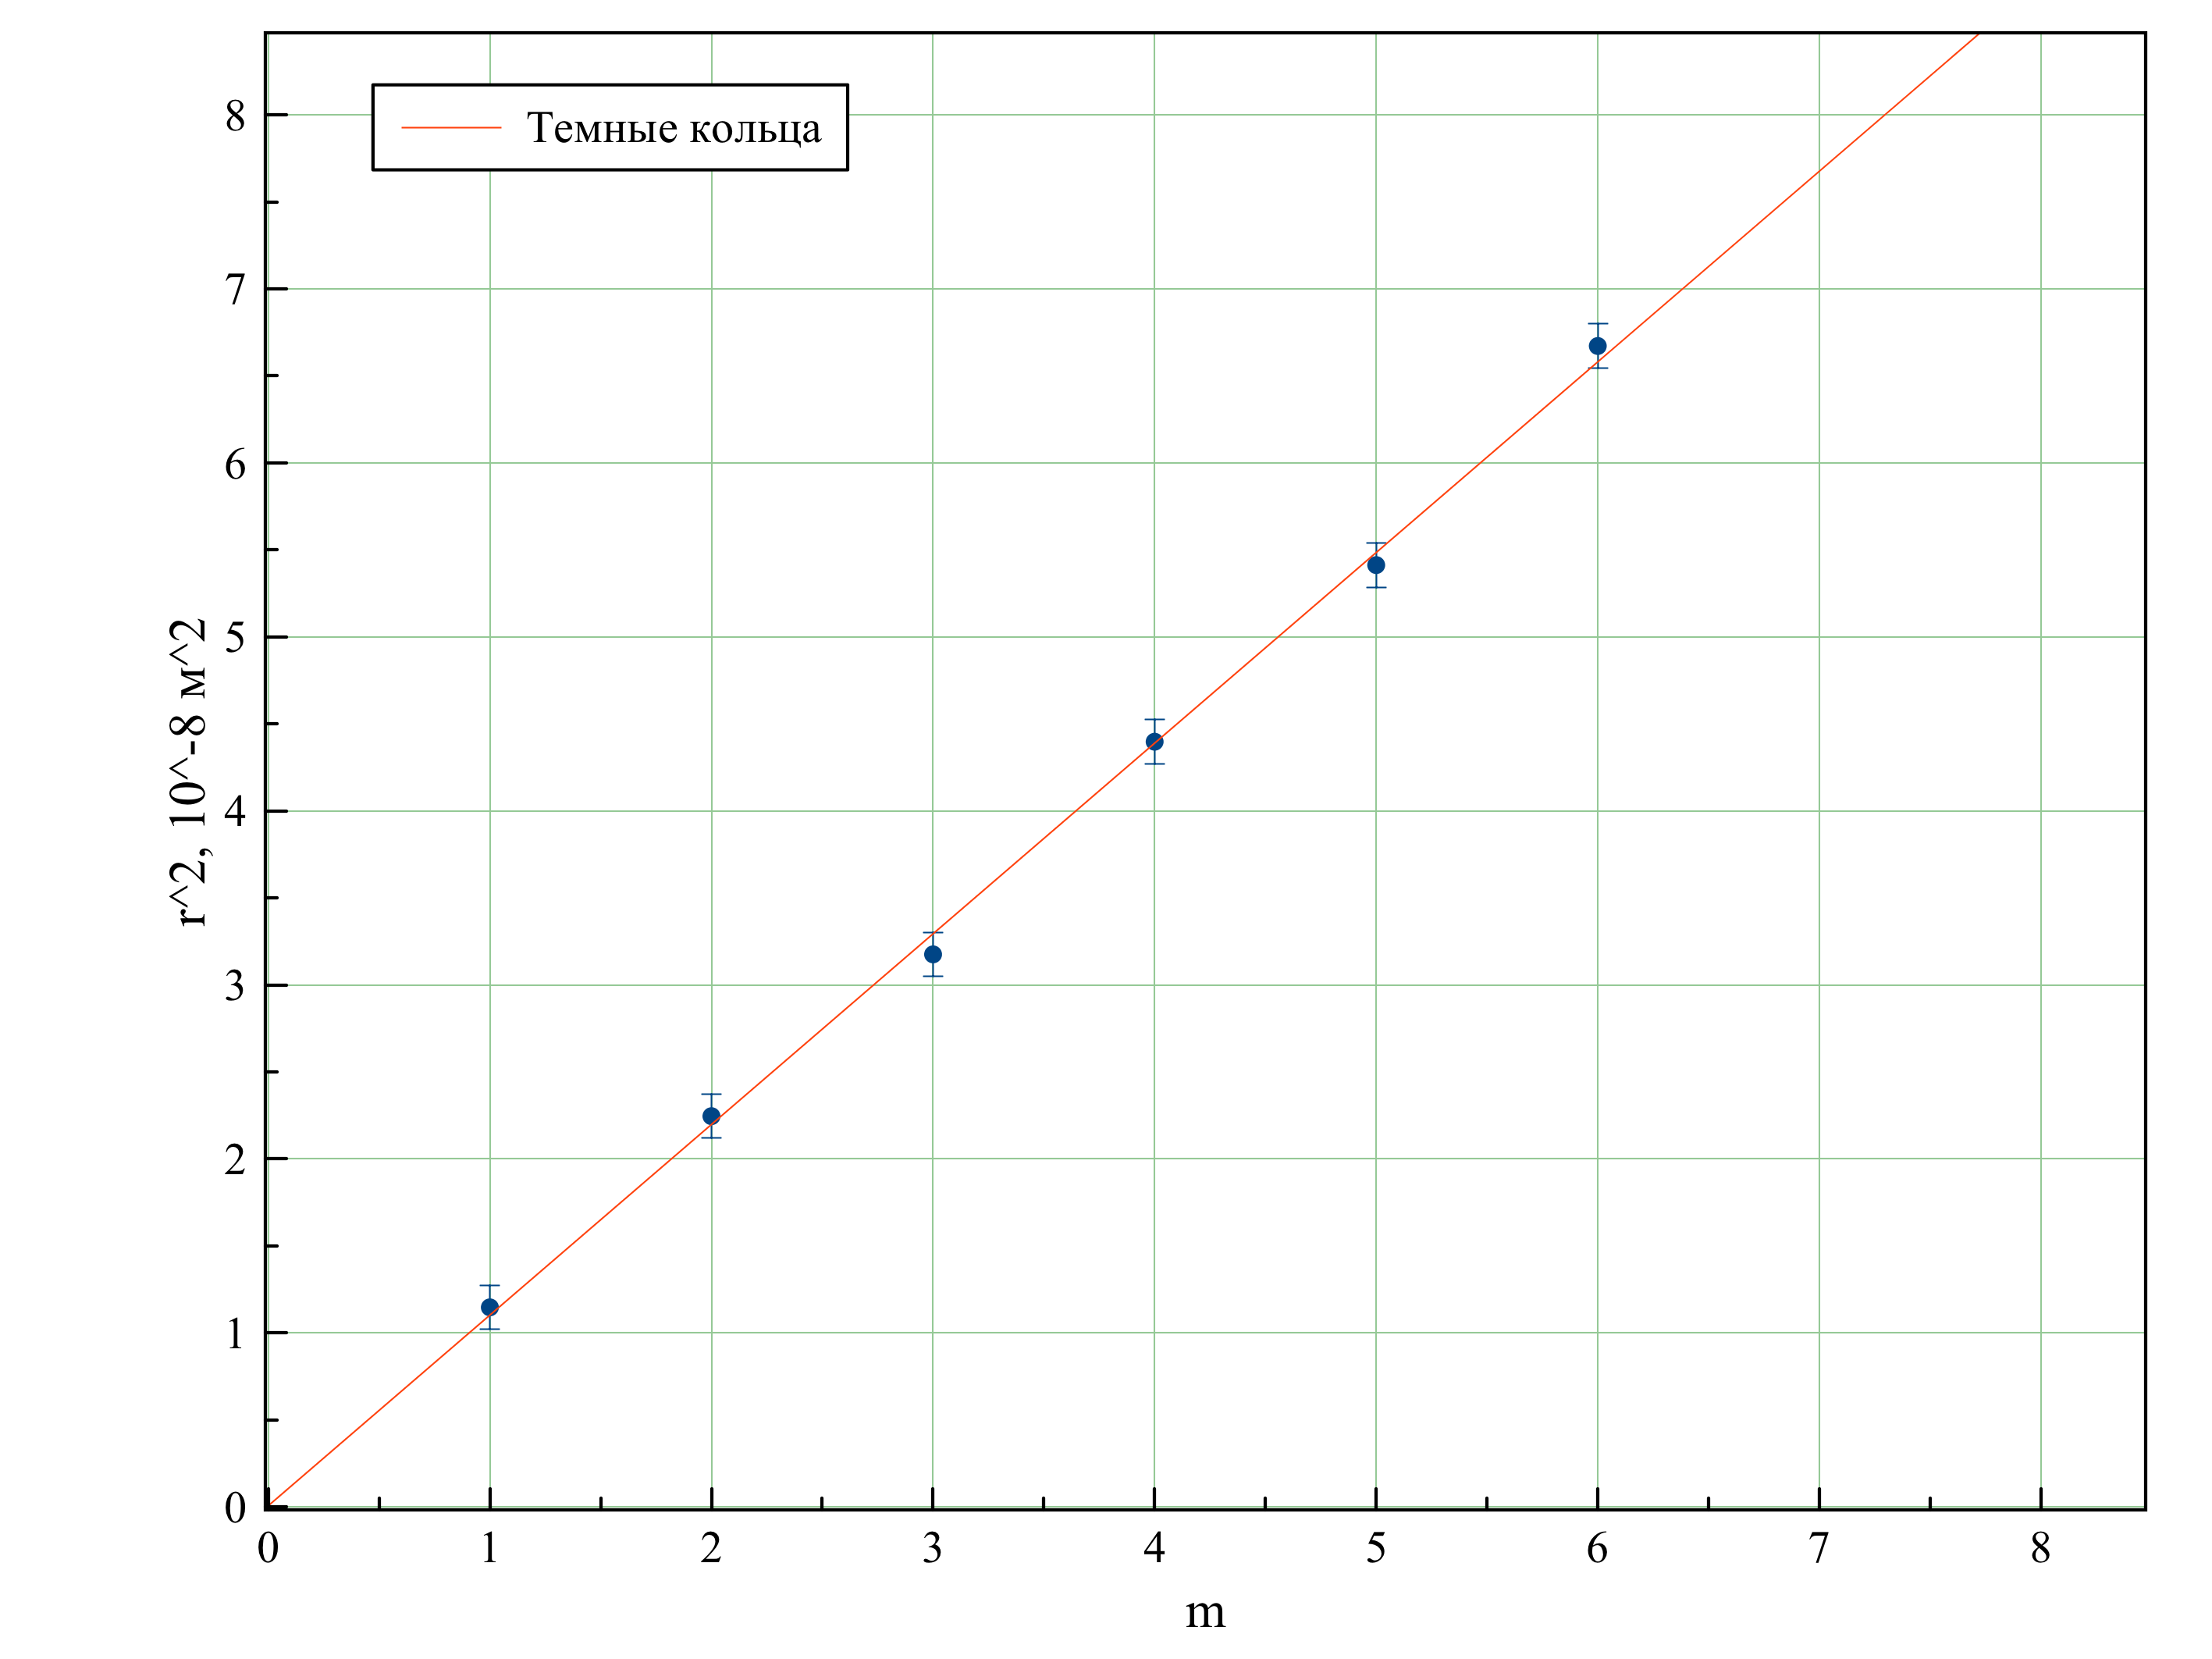
\includegraphics[width = 0.7 \lw]{dark}
\caption{График зависимости $r_m^2(m)$ для темных колец}
\end{figure}
\begin{figure}[H]
	\centering
	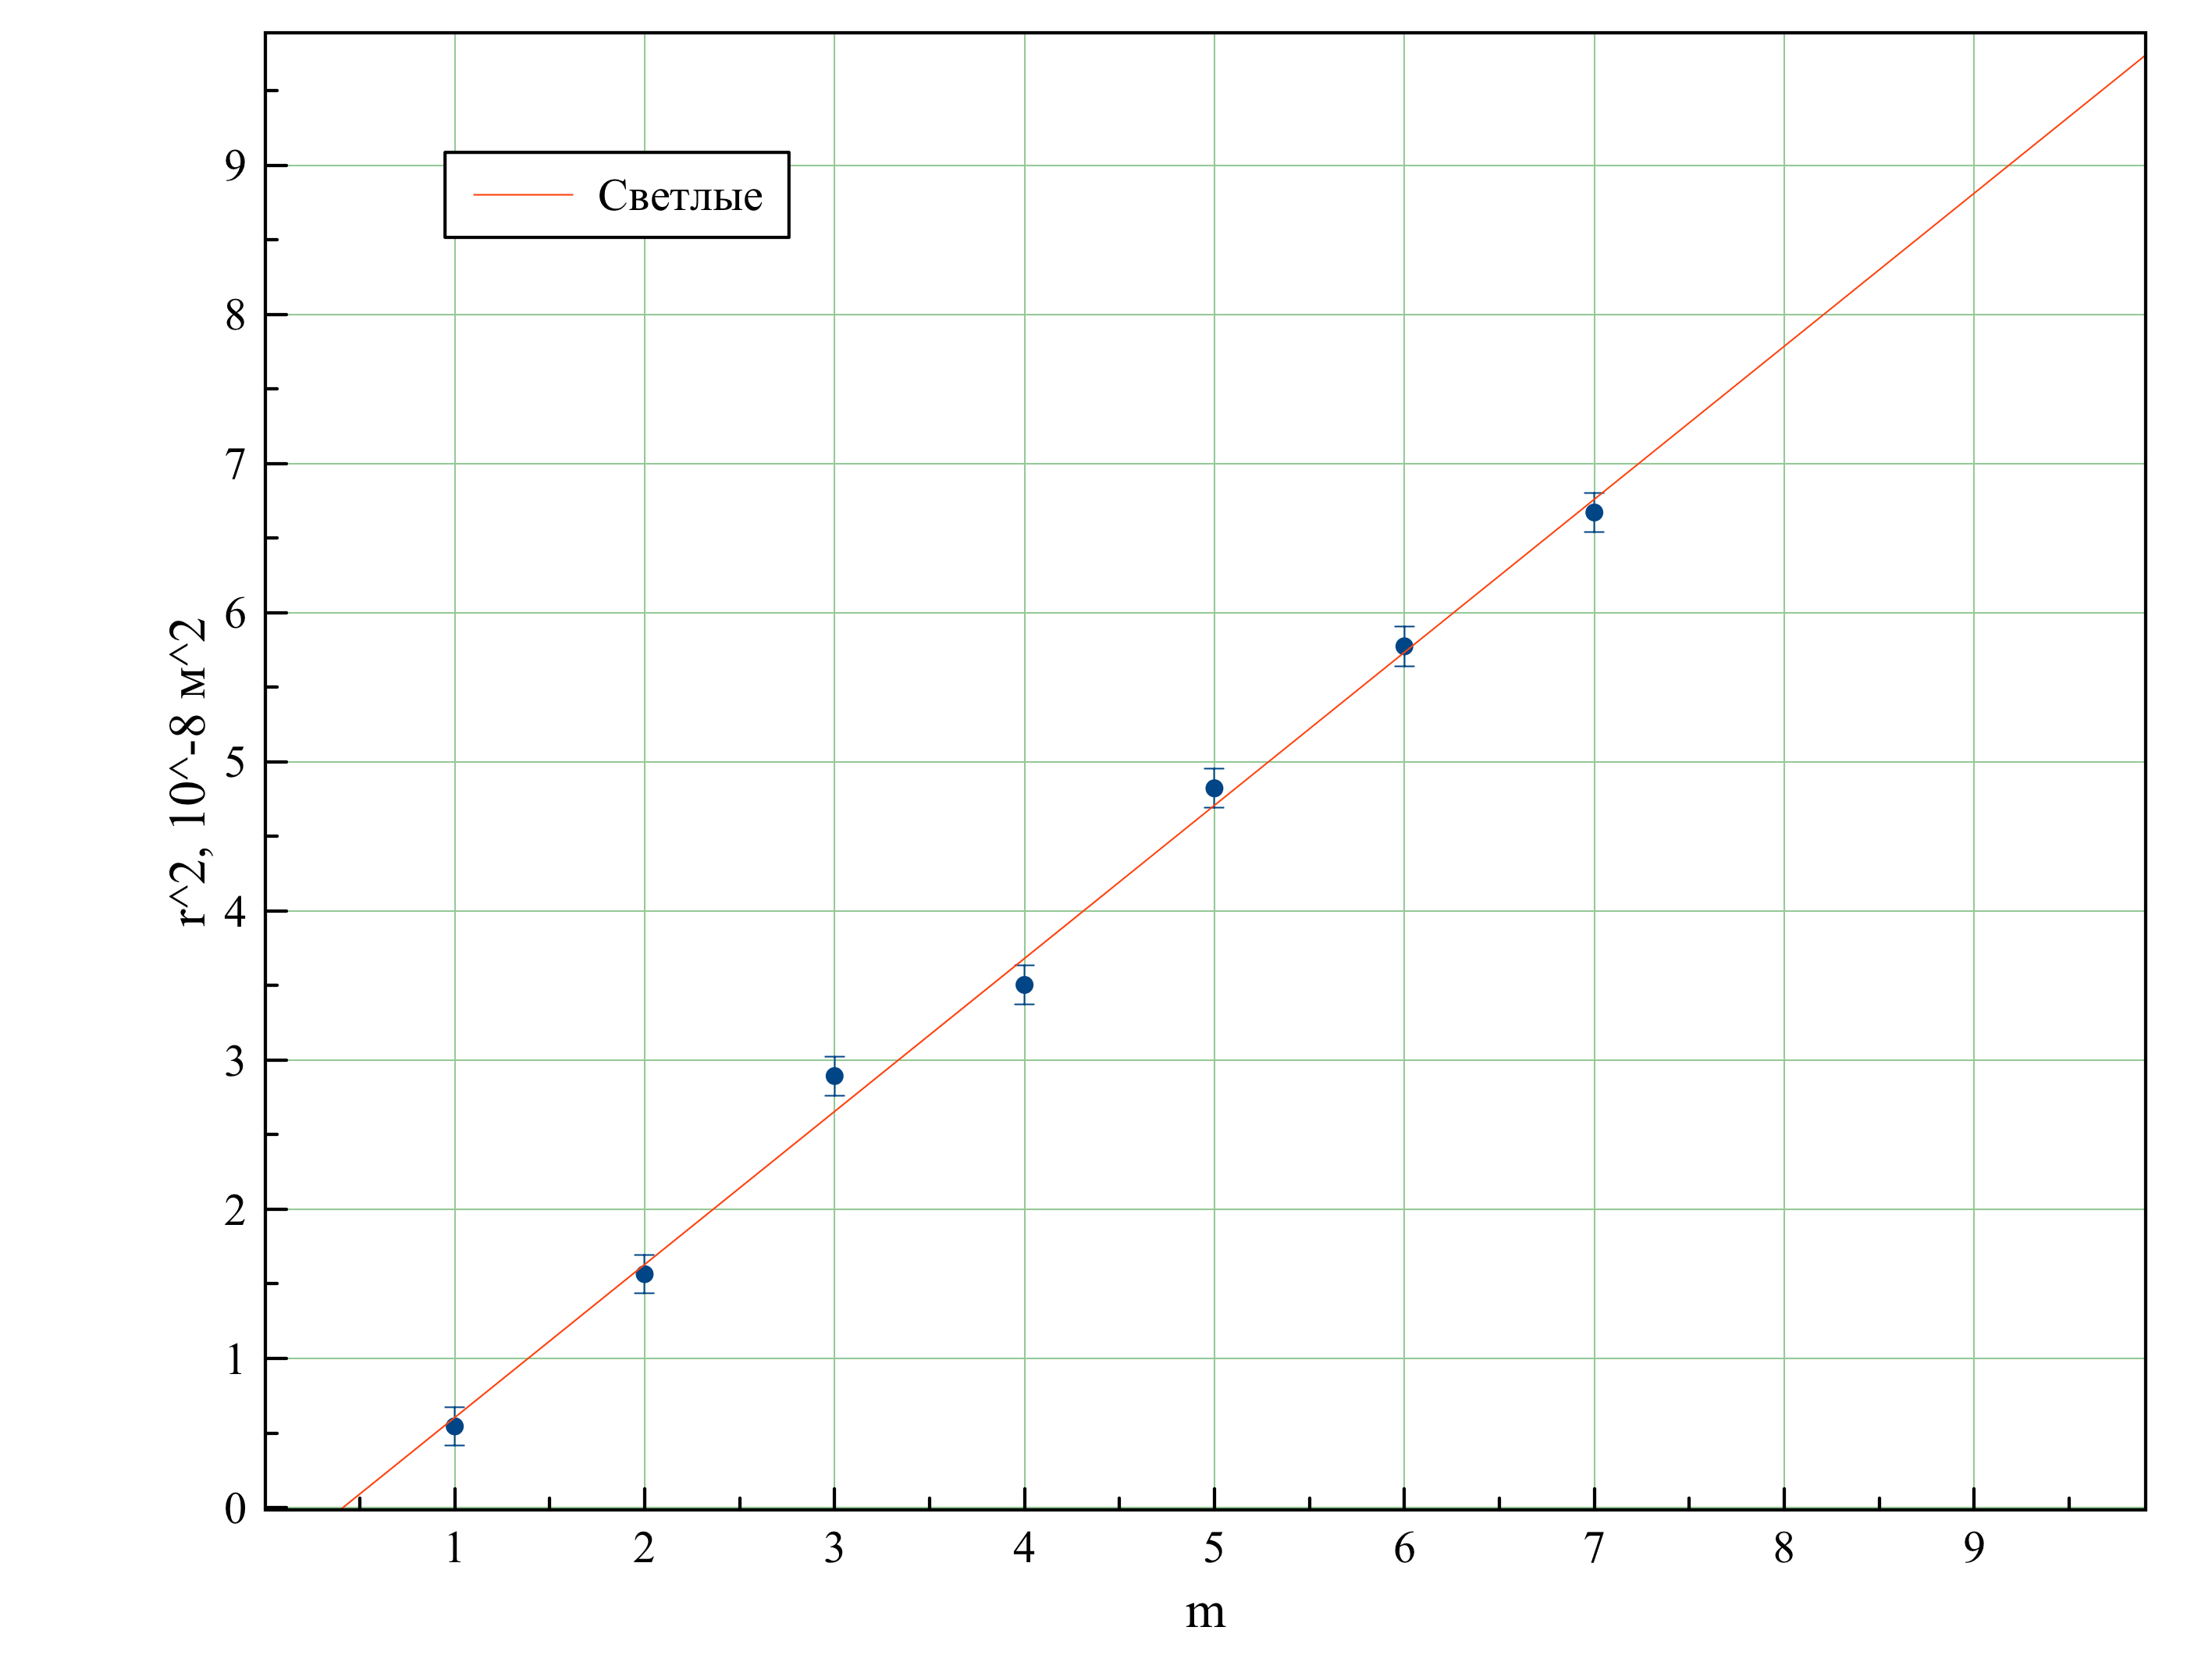
\includegraphics[width = 0.7 \lw]{light}
	\caption{График зависимости $r_m^2(m)$ для светлых колец}
\end{figure}


По наклону прямой рассчитаем радиус кривизны линзы:
\[ R = \dfrac{r^2_m}{m \lambda} = 2  \; \cm, \] где $\lambda = 546$ нм (зеленый), $\dfrac{r^2_m}{m}$ -- коэффициент наклона $1.096$

Оценим ошибку: погрешность коэффициента наклона $\sigma = 0.05 \cdot 10^{-8} \m^2$, тогда $$\sigma_R = R\cdot\left(\cfrac{\sigma_k}{k}\right) = 0.09 \cm,$$ где $k=\dfrac{r^2_m}{m}$

В итоге: \[ R \approx (2.0 \pm 0.1) \; \cm\] 

\subsection{Наблюдение биений}
Убираем монохроматор. В опак-иллюминатор поступает свет от ртутной лампы. В спектре ртутной лампы преобладают желтый и зеленый цвет. Из-за разности длин волн желтого и зеленого цвета, можно наблюдать картину биений: череду четких и нечетких систем колец.

Посчитаем количество темных полос между соседними чёткими системами: $\Delta m = 14$. Значит между центрами этих систем поместилось 14 периодов зеленого цвета и 15 желтого. Из этого можно определить длину волну желтого света:

\[ \lambda_\text{ж} = \dfrac{543 \; \n \m \cdot 15}{14} = 581 \n \m \]
Табличное значение: $\lambda_\text{ж} \approx 579 \n \m$

\section{Вывод}
Мы получили кольца Ньютона как результат интерференции света. Измерив диаметры колец, определили радиус кривизны линзы, который практически совпадает с измеренным примерно, как фокусное расстояние линзы. Более того, мы наблюдали картину биений, из периода которых определили длину волны желтого света.

\end{document}
